\documentclass{article}
\usepackage{amsfonts, amsmath, amssymb, amsthm, dsfont} % Math notations imported
\usepackage{enumitem}
\usepackage{graphicx}
\usepackage{setspace}
\usepackage{indentfirst}
\usepackage[margin=1in]{geometry}
\graphicspath{{./images/}} % Path to images

% \begin{figure}[htb!]
%      \centering
%      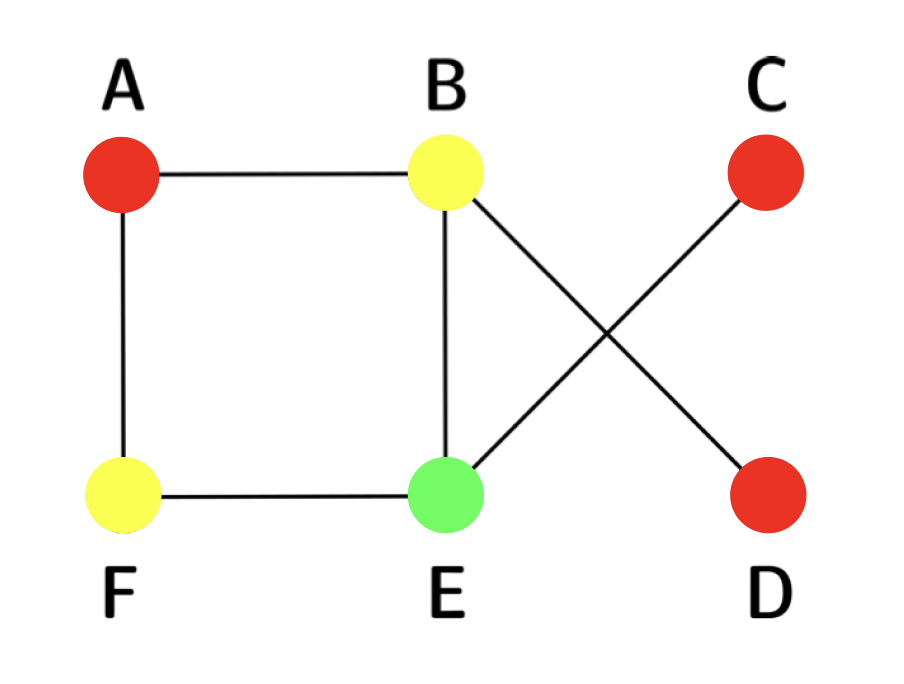
\includegraphics[scale=0.5]{coloring.png}
%      \caption{Coloring of the graph.}
% \end{figure}

% \begin{figure}[htb]
%     \qquad
%     \begin{minipage}{.4\textwidth}
%         \centering
%         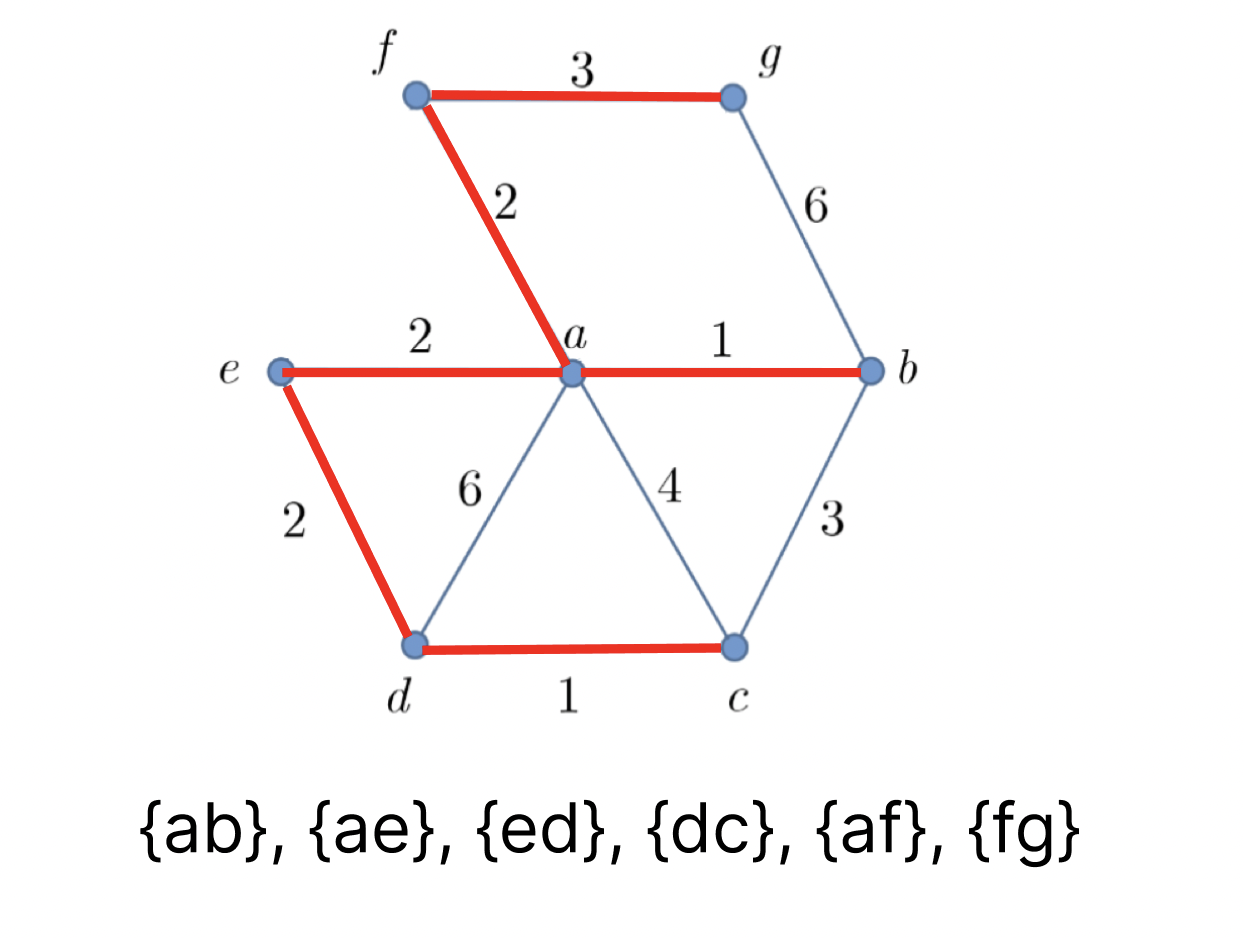
\includegraphics[scale=0.35]{prims.png}
%         \caption{}
%     \end{minipage}    
%     \qquad
%     \begin{minipage}{.4\textwidth}
%         \centering
%         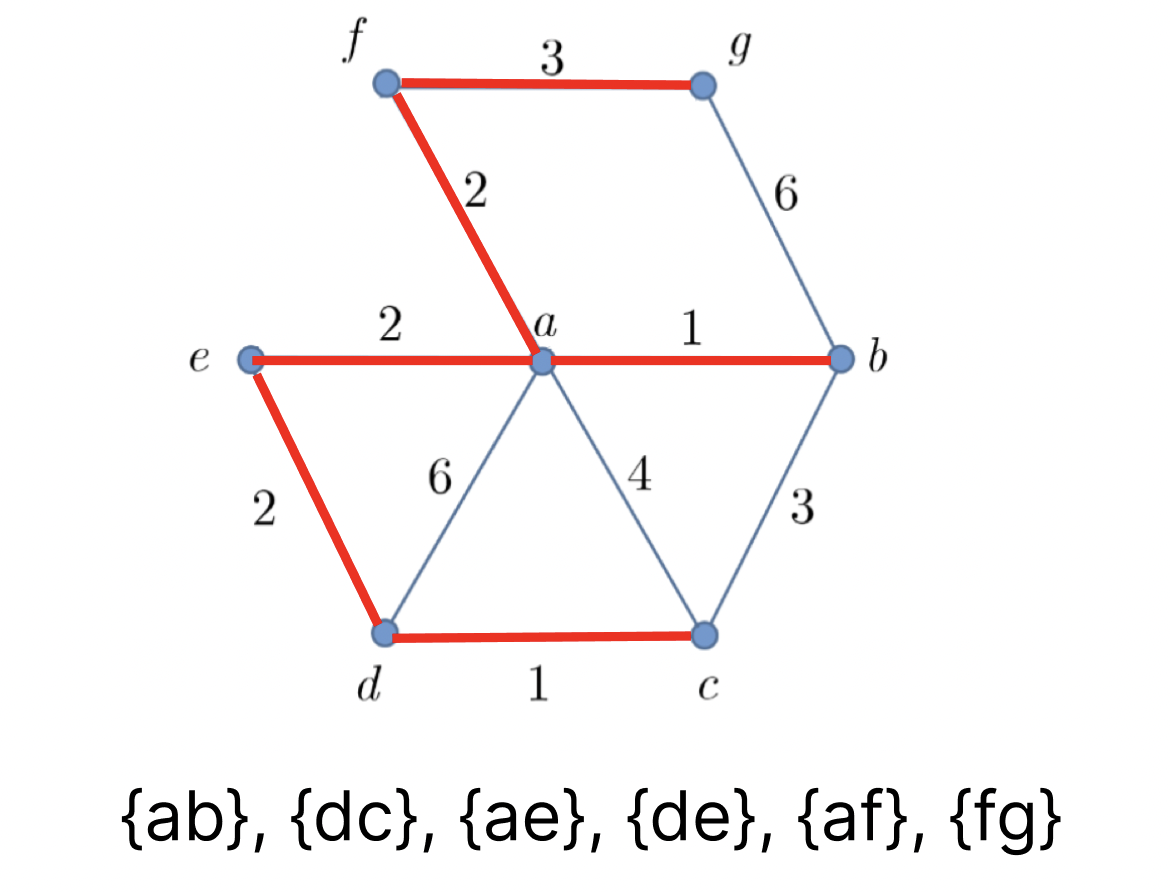
\includegraphics[scale=0.35]{kruskal.png}
%         \caption{}
%     \end{minipage}        
% \end{figure} 

\newtheorem{thm}{Theorem}
\newtheorem{proposition}[thm]{Proposition}
\newtheorem{corollary}[thm]{Corollary}
\newtheorem{lemma}[thm]{Lemma}

\newcommand*{\Var}{\ensuremath{\mathrm{Var}}}
\newcommand*{\Cov}{\ensuremath{\mathrm{Cov}}}
\newcommand*{\Corr}{\ensuremath{\mathrm{Corr}}}
\newcommand*{\Bias}{\ensuremath{\mathrm{Bias}}}
\newcommand*{\MSE}{\ensuremath{\mathrm{MSE}}}
\newcommand*{\range}{\ensuremath{\mathrm{range}}\,}
\newcommand*{\spann}{\ensuremath{\mathrm{span}}\,}
\newcommand*{\nul}{\ensuremath{\mathrm{null}}\,}
\newcommand*{\dom}{\ensuremath{\mathrm{dom}}\,}
\renewcommand*{\implies}{\ensuremath{\Longrightarrow}}
\renewcommand*{\impliedby}{\ensuremath{\Longleftarrow}}
\newcommand*{\Z}{\ensuremath{\mathbb{Z}}}
\newcommand*{\Q}{\ensuremath{\mathbb{Q}}}
\newcommand*{\R}{\ensuremath{\mathbb{R}}}
\newcommand*{\F}{\ensuremath{\mathbb{F}}}
\newcommand*{\C}{\ensuremath{\mathbb{C}}}
\newcommand*{\N}{\ensuremath{\mathbb{N}}}
\newcommand*{\E}{\ensuremath{\mathds{E}}}
\renewcommand*{\P}{\ensuremath{\mathds{P}}}
\newcommand*{\p}{\ensuremath{\mathcal{P}}}

% title information
\title{Math 110 HW9}
\author{Neo Lee}
\date{11/04/2023}

\setstretch{1.15}
% main content
\begin{document} 

% placing title information; comment out if using fancyhdr
\maketitle 

\subsection*{Problem 1.}
Suppose $V$ is a complex finite-dimensional  vector space, $T \in {\cal L}(V)$, and $\lambda \in \C$. 
Prove or disprove: if $\lambda$ is an eigenvalue of $T$, then it is also an eigenvalue of $T'$. 
Prove or disprove the converse.
\begin{proof}
    \textbf{Forward direction:}
    Let $\lambda$ be the eigenvalue, we want to show that there exists $\varphi\neq 0\in V'$ such that 
    \begin{align*}
        (T'-\lambda I)(\varphi) & = 0 \\
        T'(\varphi) - \lambda \varphi & = 0 \\
        \varphi \circ T(v) - \varphi(\lambda v) & = 0 \qquad \forall v\in V\\
        \varphi \left(T-\lambda I\right)(v) & = 0.
    \end{align*}
    Notice $(T-\lambda I)\in \mathcal{L}(V)$ is not injective because the $\nul(T-\lambda I)\neq \{0\}$, hence not surjective. Therefore, 
    $\dim \range(T-\lambda I)\le \dim V - 1$. Hence, we can construct $\varphi$ such 
    that $\varphi$ vanishes on $\range(T-\lambda I)$, and $\varphi$ is not zero. For example, 
    extend the basis of $\range(T-\lambda I)$ to the basis of $V$, denote the extended basis as 
    $\{v_1,\dots\}$, then the dual basis of $v_1$ is a suitable $\varphi$.

    \textbf{Backward direction:} We will prove by contrapositive. Suppose $\lambda$ is an 
    eigenvalue of $T'$ but not $T$, then $\nul(T-\lambda I) = \{0\}$. Thus, $T-\lambda I$ is 
    injective hence surjective, which means $\range(T-\lambda I) = V$. Therefore, there does not 
    exists $\varphi\neq 0\in V'$ such that $$\varphi \left(T-\lambda I\right)(v) = 0$$ for all $v\in V$.
    Following the above derivation (in the forward direction proof) backwards, there does not exists $\varphi\neq 0$ such that 
    $$(T'-\lambda I)(\varphi) = 0,$$ which means $\lambda$ is not an eigenvalue of $T'$.
\end{proof}

\newpage
\subsection*{Problem 2.}
Let $V$ be the complex vector space of bivariate polynomials of total degree at most $2$, and let $T$ be the linear operator 
$T : p\mapsto {\frac{\partial p}{\partial x}} -{\frac{\partial p}{\partial y}}$. 
Determine, with proof, (a) the minimal polynomial, (b) all eigenvalues, and (c) the corresponding eigenvectors of $T$.
\begin{proof}[Solution]\indent
    \begin{enumerate}[label=(\alph*)]
        \item Let $p = ax^2 + by^2 + cxy + dx + ey + f$, then 
        \begin{align*}
            T(p) & = 2ax + cy + d - 2by - cx - e = x(2a-c) + y(c-2b) + (d-e) \\
            T^2(p) & = 2a - c - c + 2b = 2a + 2b - 2c \\
            T^3(p) & = 0.
        \end{align*}
        Notice the minimal polynomial must be of degree at least 3 because $I(p), T(p), T^2(p)$ are 
        linearly independent due to different degrees. In fact, the minimal polynomial is of degree 
        3 because $T^3(p) = 0$. Therefore, the coefficients for the minimal polynomial satisfy
        \begin{align*}
            T^3(p) + \beta T^2(p) + \gamma T(p) + \delta I(p) & = 0 \\
            \beta T^2(p) + \gamma T(p) + \delta I(p) & = 0 \\
            \implies \beta = \gamma = \delta & = 0.
        \end{align*}
        Hence, the minimal polynomial is $q(z)=z^3$.
        
        \item By \emph{Theorem 5.27}, the eigenvalues of $T$ are the zeros of the minimal polynomial,
        hence the only eigenvalues are $0$.

        \item We want to find $E(0, T)$.
        \begin{align*}
            T(p) & = 0= x(2a-c) + y(c-2b) + (d-e) \\
            & \implies \begin{cases}
                2a-c = 0 \\
                c-2b = 0 \\
                d-e = 0
            \end{cases} \\
            & \implies \begin{cases}
                a = b = \frac{c}{2} \\
                d = e.
            \end{cases}
        \end{align*}
        Hence, \begin{align*}
            p & = cx^2 + cy^2 + 2cxy + dx + dy + f \\
            & = c(x+y)^2 + d(x+y) + f \\
            & \implies E(0, T) = \spann\{1, x+y, (x+y)^2\}.
        \end{align*}
        The corresponding eigenvectors are $\{1, x+y, (x+y)^2\}$.
    \end{enumerate}

\end{proof}

\newpage
\subsection*{Problem 3.}
Suppose $V$ is a finite-dimensional vector space. Prove or disprove: if two linear operators
$T$ and $S$ from ${\cal L} (V)$ commute, then $T$ is diagonalizable if and only if $S$ is.
\begin{proof}[Solution]
    We will provide a counter example. Consider $V=\p_2(\R)$, $S = I$ and $T = D$, the differentiation
    operator. Obviously, $ID = DI$, and $S$ is diagonalizable, but $T$ is not because 
    all non-zero vectors in $V$ will be reduced by one degree after mapping with $T$, hence no non-zero
    vectors is a scalar multiple itself after mapping with $T$.
\end{proof}

\newpage
\subsection*{Problem 4.}
Let $V := {\cal P}_3(\R)$ and let $T\in {\cal L}(V)$ be the operator $f(x)\mapsto f(x-1)+f(x+1)$. 
Is $T$ triangularizable? If yes, is $T$ also diagonalizable? Justify your answers.
\begin{proof}[Solution]
    Let $f = ax^3 + bx^2 + cx + d$, then 
    \begin{align*}
        T(f) & = a(x-1)^3 + b(x-1)^2 + c(x-1) + d + a(x+1)^3 + b(x+1)^2 + c(x+1) + d \\
        & = 2ax^3 + 2bx^2 + (6a + 2c)x + (2b+2d).
    \end{align*}
    Hence, the matrix representation of $T$ with respect to $(x^3,x^2,x,1)$ is
    $$\mathcal{M}(T) = \begin{bmatrix}
        2 & 0 & 0 & 0 \\
        0 & 2 & 0 & 0 \\
        6 & 0 & 2 & 0 \\
        0 & 2 & 0 & 2
    \end{bmatrix},$$
    which is already triangular. Therefore, $T$ is triangularizable. 
    
    However, $T$ is not diagonalizable. By \emph{Theorem 5.41}, the eigenvalues of $T=\{2\}$. 
    Then we want to find the eigenspace $E(2,T)$,
    \begin{align*}
        T(f) = 2ax^3 + 2bx^2 + (6a + 2c)x + (2b+2d) & = 2ax^3 + 2bx^2 + 2cx + 2d \\
        (6a+2c)x + (2b + 2d) & = 2cx + 2d
    \end{align*}
    \begin{align*}
        \implies & \begin{cases}
            6a + 2c = 2c \\
            2b + 2d = 2d
        \end{cases} \\
        \implies & \begin{cases}
            a = 0 \\
            b = 0.
        \end{cases}
    \end{align*}
    Hence, $E(2,T) = \spann\{x, 1\}$, which does not span $\p_3(\R)$. Therefore, 
    $T$ is not diagonalizable.
\end{proof}

\newpage
\subsection*{Problem 5.}
Determine whether or not the function taking the pair $((x_1,x_2,x_3),(y_1,y_2,y_3)) \in \R^3 
\times \R^3$ to $x_1y_1+x_2y_2-3x_2y_3+3x_3y_2+x_3y_3$ is an inner product. 
\begin{proof}
    \textbf{Positivity:} Let $v = (a,b,c)$, 
    $$\langle v,v\rangle = a^2+b^2 - 3bc + 3bc + c^2 = a^2 + b^2 + c^2 \ge 0.$$

    \textbf{Definiteness:} Let $v= (a,b,c)$,
    \begin{align*}
        \langle v,v\rangle & = 0 \\
        a^2+b^2+c^2 & = 0 \\
        & \implies a^2 = b^2 = c^2 = 0 \\
        & \implies a = b = c = 0.
    \end{align*}

    \textbf{Additivity in first slot:} Let $u=(a_1,b_1,c_1), v=(a_2,b_2,c_2), w=(a_3,b_3,c_3)$,
    \begin{align*}
        \langle u+v, w\rangle & = (a_1+a_2)(a_3) + (b_1+b_2)(b_3) + (c_1+c_2)(c_3) - 3(b_1+b_2)(c_3) + 3(c_1+c_2)(b_3) \\
        & = (a_1a_3 + b_1b_3 + c_1c_3 - 3b_1c_3 + 3c_1b_3) + (a_2a_3 + b_2b_3 + c_2c_3 - 3b_2c_3 + 3c_2b_3) \\
        & = \langle u,w\rangle + \langle v,w\rangle.
    \end{align*}

    \textbf{Homogeneity in first slow:} Let $u=(a_1,b_1,c_1), v=(a_2,b_2,c_2)$,
    \begin{align*}
        \langle \lambda u, w\rangle & = \lambda a_1a_2 + \lambda b_1b_2 + \lambda c_1c_2 - 3\lambda b_1c_2 + 3\lambda c_1b_2 \\
        & = \lambda (a_1a_2 +  b_1b_2 +  c_1c_2 - 3 b_1c_2 + 3 c_1b_2) \\
        & = \lambda \langle u,w\rangle.
    \end{align*}

    \textbf{Conjugate symmetry:} Let $u=(1,2,3), v=(4,5,6)$,
    \begin{align*}
        \langle u,v\rangle & = 1\times 4 + 2\times 5 + 3\times 6 - 3\times 2\times 6 + 3\times 3\times 5 \\
        & \neq 1\times 4 + 2\times 5 + 3\times 6 - 3\times 3\times 5 + 3\times 2\times 6 = \langle v, u\rangle.
    \end{align*}

    Hence, the function is not an inner product.
\end{proof}

\end{document}
